\documentclass{standalone}
\usepackage{graphicx}	
\usepackage{amssymb, amsmath}
\usepackage{color}

\usepackage{tikz}
\usetikzlibrary{intersections, backgrounds, math, decorations.pathreplacing}
\usepackage{pgfmath}

\definecolor{light}{RGB}{220, 188, 188}
\definecolor{mid}{RGB}{185, 124, 124}
\definecolor{dark}{RGB}{143, 39, 39}
\definecolor{highlight}{RGB}{180, 31, 180}
\definecolor{lightteal}{RGB}{186, 219, 219}
\definecolor{midteal}{RGB}{124, 186, 186}
\definecolor{darkteal}{RGB}{38, 142, 142}
\definecolor{darkerteal}{RGB}{0, 124, 124}
\definecolor{gray10}{gray}{0.1}
\definecolor{gray20}{gray}{0.2}
\definecolor{gray30}{gray}{0.3}
\definecolor{gray40}{gray}{0.4}
\definecolor{gray60}{gray}{0.6}
\definecolor{gray70}{gray}{0.7}
\definecolor{gray80}{gray}{0.8}
\definecolor{gray90}{gray}{0.9}
\definecolor{gray95}{gray}{0.95}

\begin{document}

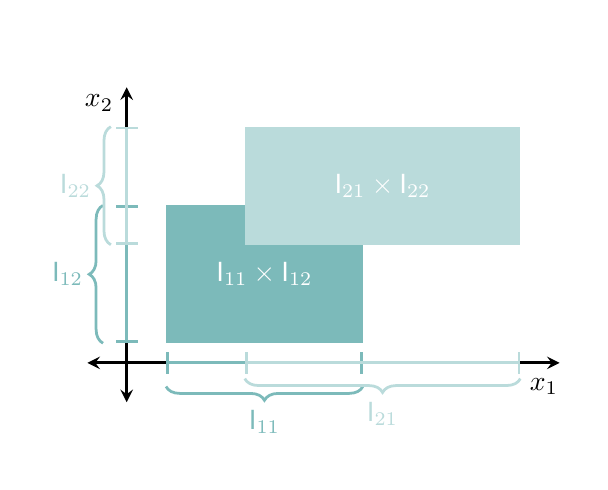
\begin{tikzpicture}[scale=1.0]

  \pgfmathsetmacro{\xa}{-2};
  \pgfmathsetmacro{\xb}{0.5};
  \pgfmathsetmacro{\ya}{-1.25};
  \pgfmathsetmacro{\yb}{0.5};

  \pgfmathsetmacro{\Xa}{-1};
  \pgfmathsetmacro{\Xb}{2.5};
  \pgfmathsetmacro{\Ya}{0};
  \pgfmathsetmacro{\Yb}{1.5};
  
  \draw[white] (-3.75, -2.75) rectangle (3.25, 2.75);
  
  \draw [<->, >=stealth, line width=1] (-2.5, -2) -- +(0, 4);
  \draw [<->, >=stealth, line width=1] (-3, -1.5) -- +(6, 0);
  
  \node at (2.8, -1.8) { $x_{1}$ };
  \node at (-2.85, 1.8) { $x_{2}$ };
  
  \draw[|-|, midteal, line width=1] (\xa, -1.5) -- (\xb, -1.5);
  \draw[decorate,decoration={brace,amplitude=5pt}, midteal, line width=1] (\xb, -1.8) -- (\xa, -1.8);
  \node[midteal] at ( { 0.5 * ( \xa + \xb) }, -2.25) { $\mathsf{I}_{11}$ };
 
  \draw[|-|, midteal, line width=1] (-2.5, \ya) -- (-2.5, \yb);
  \draw[decorate,decoration={brace,amplitude=5pt}, midteal, line width=1] (-2.8, \ya) -- (-2.8, \yb);
  \node[midteal] at ( -3.25, { 0.5 * ( \ya + \yb) } ) { $\mathsf{I}_{12}$ };
  
  \fill[midteal] (\xa, \ya) rectangle (\xb, \yb) 
  node[white, midway] { $\mathsf{I}_{11} \times \mathsf{I}_{12}$ };

  \draw[|-|, lightteal, line width=1] (\Xa, -1.5) -- (\Xb, -1.5);
  \draw[decorate,decoration={brace,amplitude=5pt}, lightteal, line width=1] (\Xb, -1.7) -- (\Xa, -1.7);
  \node[lightteal] at ( { 0.5 * ( \Xa + \Xb) }, -2.15) { $\mathsf{I}_{21}$ };
 
  \draw[|-|, lightteal, line width=1] (-2.5, \Ya) -- (-2.5, \Yb);
  \draw[decorate,decoration={brace,amplitude=5pt}, lightteal, line width=1] (-2.7, \Ya) -- (-2.7, \Yb);
  \node[lightteal] at ( -3.15, { 0.5 * ( \Ya + \Yb) } ) { $\mathsf{I}_{22}$ };
  
  \fill[lightteal] (\Xa, \Ya) rectangle (\Xb, \Yb) 
  node[white, midway] { $\mathsf{I}_{21} \times \mathsf{I}_{22}$ };
  
\end{tikzpicture}

\end{document}  